\chapter{Measuring Time}\label{ch:g2:measuring-time}

``Just five more minutes!'' --- but how long is that, really? Time
cannot be seen, held, or laid along a ruler. And yet we \omterm{def:g2:measuring-length:measure}{measure} it
every day: races have winners, cakes come out neither raw nor burnt,
and school ends at the right moment. Let us learn how time is tamed.

\section{Moments and durations}

\begin{example}[The order of the day]\label{ex:g2:measuring-time:order}
A day is a parade of events, always in order: wake up, breakfast,
school, lunch, afternoon, dinner, bed. ``Breakfast comes
\emph{before} school'' and ``dinner comes \emph{after} lunch'' ---
before and after are the first words of time, just as longer and
shorter were the first words of length.
\end{example}

\begin{omfigure}
\begin{tikzpicture}[scale=0.85]
  \draw[-Stealth, very thick] (0,0) -- (11.4,0);
  \foreach \x/\name in {0.8/wake up, 2.9/breakfast, 5.0/school,
      7.1/lunch, 9.2/dinner, 10.7/bed} {
    \fill[omDef] (\x,0) circle (2.4pt);
    \node[above, font=\small, rotate=40, anchor=south west]
      at (\x,0.15) {\name};
  }
\end{tikzpicture}

{\small One day laid out like a number line: each event has its
place, and the arrow shows which way time flows --- always forward.}
\end{omfigure}

\begin{definition}[Duration]\label{def:g2:measuring-time:duration}
A \emph{moment}\index{moment} is one point of the day: the moment the
bell rings. A \emph{duration}\index{duration} is the stretch of time
between two moments: from the bell to the end of the lesson. Moments
answer \emph{when?}; durations answer \emph{how long?}
\end{definition}

\begin{example}[When or how long?]\label{ex:g2:measuring-time:whenhowlong}
``The film starts after dinner'' talks about a moment. ``The film
lasts as long as two lunch breaks'' talks about a \omterm{def:g2:measuring-time:duration}{duration}. ``My
birthday is in spring'': moment. ``The holidays felt so short'':
\omterm{def:g2:measuring-time:duration}{duration} --- and this chapter is mostly about \omterm{def:g2:measuring-time:duration}{durations}.
\end{example}

\section{Comparing durations}

\begin{method}[A fair race of durations]\label{met:g2:measuring-time:race}
To find which of two things lasts longer:
\begin{enumerate}
  \item start both at the \emph{same moment} --- ``ready, set, go!'';
  \item watch which one finishes first;
  \item the one still going when the other has finished lasts longer.
\end{enumerate}
If they cannot run together (today's bath and yesterday's dinner),
race each of them against the \emph{same} third thing --- a sand
timer.
\end{method}

\begin{example}[The sand timer]\label{ex:g2:measuring-time:sandtimer}
A sand timer is a little glass with a narrow waist: the sand always
takes the \emph{same} \omterm{def:g2:measuring-time:duration}{duration} to pour through. That makes it a
referee. Brushing your teeth against the timer: the sand ran out
first --- brush longer! A song against the timer: the song won. So
the song lasts longer than the tooth-brushing, though they never
raced each other directly.
\end{example}

\begin{omfigure}
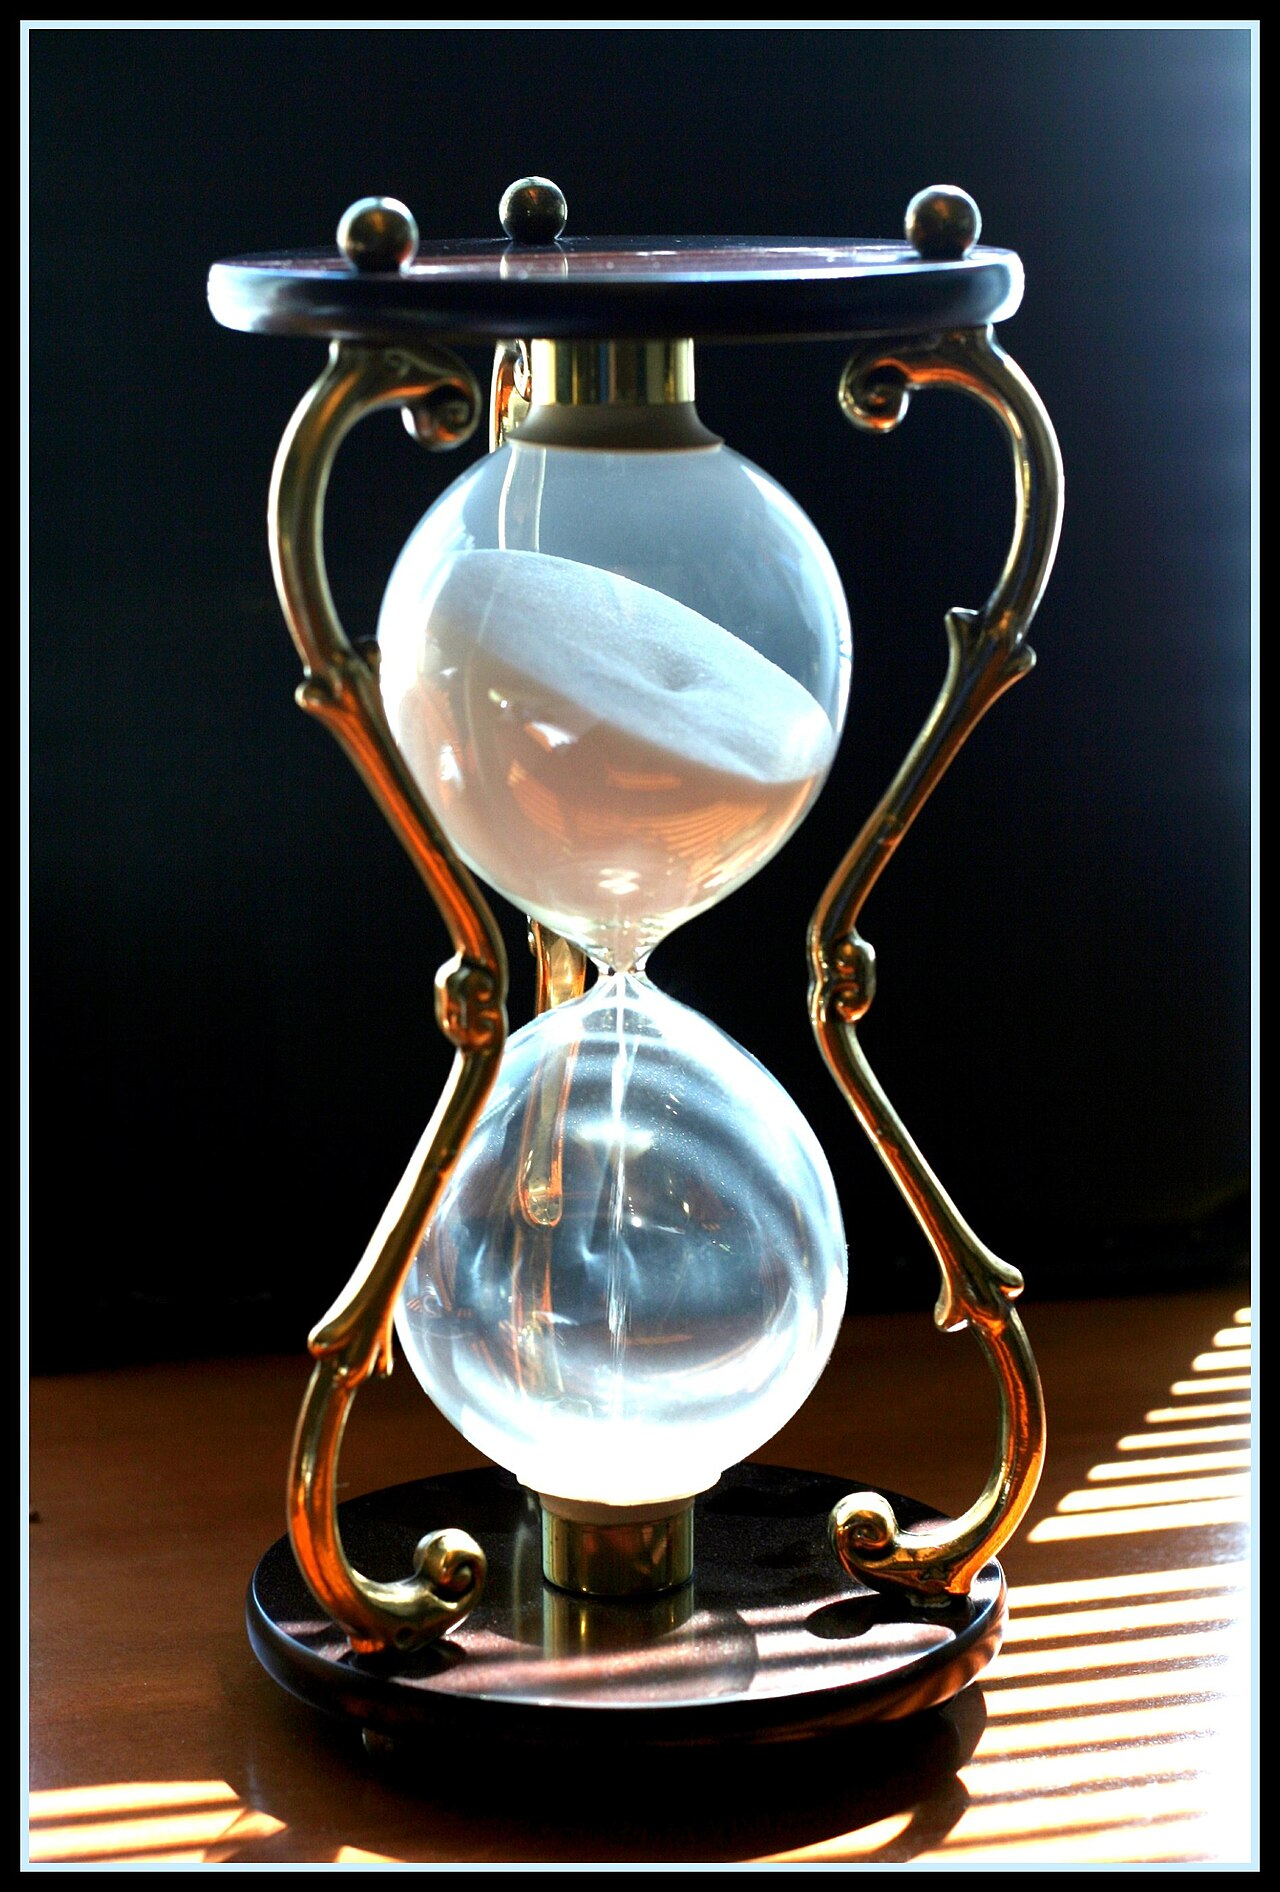
\includegraphics[width=0.34\linewidth]{images/book1/hourglass.jpg}

{\small A sand timer: a \omterm{def:g2:measuring-time:duration}{duration} you can hold in your hand. The
sand always needs the same time to slip through the narrow waist ---
turn it over, and it referees again. \emph{Photo: John Morgan,
CC BY 2.0.}}
\end{omfigure}

\begin{remark}[Feelings are bad clocks]\label{rem:g2:measuring-time:feelings}
A fun afternoon flies; a boring queue crawls --- yet the clock may
count the same for both. Our sense of time is easily fooled, just as
touch was fooled about hot and cold. That is exactly why referees
like the sand timer matter: sand does not get bored.
\end{remark}

\section{Counting steady beats}

\begin{definition}[The second]\label{def:g2:measuring-time:second}
The \emph{second}\index{second} is the \omterm{def:g2:measuring-length:measure}{unit} of time used all over
the world, written \unit{s}. One second is about one calm heartbeat,
or the steady tick of a big clock. Saying ``one little crocodile,
two little crocodiles'' at a calm pace counts roughly one second per
crocodile.
\end{definition}

\begin{example}[Try it: how many seconds?]\label{ex:g2:measuring-time:count}
Count seconds steadily while: you hold your breath comfortably; the
tap fills a glass; a friend runs to the fence and back. The glass
might take $6$ seconds, the run $20$. Now the tooth-brushing and the
song from before can get \emph{numbers} --- and numbers, as with
lengths, can travel and be checked.
\end{example}

\begin{example}[Hours on the clock]\label{ex:g2:measuring-time:clock}
Seconds are for short things. Long stretches are counted in
\emph{hours}\index{hour}: school mornings last \omterm{ex:g2:measuring-time:clock}{hours}, a night of
sleep too. The clock's short hand points to the hour: straight at
the $3$, it is three o'clock; between $3$ and $4$ with the long hand
pointing straight down, it is half past three. A whole day and night
together hold $24$ \omterm{ex:g2:measuring-time:clock}{hours} --- while the Earth, remember, makes one
full turn.
\end{example}

\begin{omfigure}
\begin{tikzpicture}[scale=0.85]
  \draw[thick] (0,0) circle (1.5);
  \foreach \h in {1,...,12} {
    \node[font=\footnotesize] at ({90-\h*30}:1.22) {\h};
  }
  \draw[very thick, omDef] (0,0) -- ({90-3*30}:0.8);
  \draw[thick, omThm] (0,0) -- (90:1.05);
  \node[below, font=\small] at (0,-1.75) {three o'clock};
  \begin{scope}[xshift=6cm]
    \draw[thick] (0,0) circle (1.5);
    \foreach \h in {1,...,12} {
      \node[font=\footnotesize] at ({90-\h*30}:1.22) {\h};
    }
    \draw[very thick, omDef] (0,0) -- ({90-3.5*30}:0.8);
    \draw[thick, omThm] (0,0) -- (270:1.05);
    \node[below, font=\small] at (0,-1.75) {half past three};
  \end{scope}
\end{tikzpicture}

{\small Two clocks: the short hand tells the hour. At half past
three, it has walked halfway from the $3$ toward the $4$.}
\end{omfigure}

\section{Exercises}

\begin{exercise}[$\star$]\label{exo:g2:measuring-time:1}
Put in order: dinner; \ wake up; \ afternoon playtime; \ breakfast;
\ bed.
\end{exercise}

\begin{exercise}[$\star$]\label{exo:g2:measuring-time:2}
Moment or \omterm{def:g2:measuring-time:duration}{duration}? ``The bell rings at noon''; \ ``the cake bakes
for half an hour''; \ ``we left after lunch''; \ ``the trip felt
endless''.
\end{exercise}

\begin{exercise}[$\star$]\label{exo:g2:measuring-time:3}
Two candles are lit at the same moment; the red one goes out while
the blue one still burns. Which candle lasted longer? Which rule of
\cref{met:g2:measuring-time:race} did the candles follow?
\end{exercise}

\begin{exercise}[$\star$]\label{exo:g2:measuring-time:4}
Why is a sand timer a fair referee for \omterm{def:g2:measuring-time:duration}{durations}? What is always the
same about it, every time it is turned?
\end{exercise}

\begin{exercise}[$\star$]\label{exo:g2:measuring-time:5}
Ben says his boring wait at the dentist lasted ``forever''. His
watch says it lasted less than his favorite cartoon. How is this
possible? (See \cref{rem:g2:measuring-time:feelings}.)
\end{exercise}

\begin{exercise}[$\star$]\label{exo:g2:measuring-time:6}
Count seconds steadily and \omterm{def:g2:measuring-length:measure}{measure}: how many seconds does it take
you to write your full name? To put on your shoes?
\end{exercise}

\begin{exercise}[$\star$]\label{exo:g2:measuring-time:7}
Which \omterm{def:g2:measuring-length:measure}{unit} fits better, seconds or \omterm{ex:g2:measuring-time:clock}{hours}: a sneeze; \ a night of
sleep; \ tying a shoelace; \ a school morning?
\end{exercise}

\begin{exercise}[$\star$]\label{exo:g2:measuring-time:8}
Draw a clock showing five o'clock, and another showing half past
five. Where does the short hand point at half past five?
\end{exercise}

\begin{exercise}[$\star\star$]\label{exo:g2:measuring-time:9}
Yesterday's bath and today's shower cannot race each other. Explain,
step by step, how to find out which lasts longer using one sand
timer --- and what to write down so your friend can check.
\end{exercise}

\begin{exercise}[$\star\star$]\label{exo:g2:measuring-time:10}
Lila counts ``one, two, three\dots'' very fast and says the glass
filled in $12$ seconds; Tom counts calmly and finds $6$. The tap ran
the same both times. Who is closer to the truth, and what makes
counting seconds honest?
\end{exercise}
